% ============================================================
%  ITU UCK 427E
%  Oxidation Pathways: CH4, H2, Aerospace Fuels
%  Beamer -- custom dark theme, pdflatex compatible
% ============================================================
\documentclass[aspectratio=169,10pt]{beamer}

\usepackage[utf8]{inputenc}
\usepackage[T1]{fontenc}
\usepackage{amsmath,amssymb}
\usepackage[version=4]{mhchem}
\usepackage{tikz}
\usetikzlibrary{arrows.meta,positioning,shapes.geometric,calc,backgrounds,fit}
\usepackage{booktabs}
\usepackage{colortbl}
\usepackage{xcolor}
\usepackage{microtype}
\usepackage{pgfplots}
\pgfplotsset{compat=1.18}
\usepackage{array}
\usepackage{multirow}
\usepackage{helvet}
\renewcommand{\familydefault}{\sfdefault}

% ── Colour palette ─────────────────────────────────────────
\definecolor{ITUnavy}{HTML}{0D1B2A}
\definecolor{ITUsteel}{HTML}{1B3A5C}
\definecolor{ITUsky}{HTML}{2E86AB}
\definecolor{ITUorange}{HTML}{E86B2C}
\definecolor{ITUgold}{HTML}{F4A261}
\definecolor{ITUcream}{HTML}{F0EBE3}
\definecolor{ITUgreen}{HTML}{1E8449}
\definecolor{ITUred}{HTML}{C0392B}
\definecolor{ITUmuted}{HTML}{8A9BB0}
\definecolor{ITUpanel}{HTML}{112030}
\definecolor{ITUlight}{HTML}{D6E4EE}

% ── Theme setup ────────────────────────────────────────────
\useoutertheme[footline=authorinstitutetitle]{miniframes}
\useinnertheme{rectangles}

\setbeamercolor{background canvas}{bg=ITUnavy}
\setbeamercolor{normal text}{fg=ITUcream,bg=ITUnavy}
\setbeamercolor{structure}{fg=ITUsky}
\setbeamercolor{frametitle}{bg=ITUsteel,fg=white}
\setbeamercolor{title}{fg=white,bg=ITUnavy}
\setbeamercolor{subtitle}{fg=ITUgold}
\setbeamercolor{section in head/foot}{bg=ITUsteel,fg=ITUlight}
\setbeamercolor{subsection in head/foot}{bg=ITUnavy,fg=ITUmuted}
\setbeamercolor{itemize item}{fg=ITUorange}
\setbeamercolor{itemize subitem}{fg=ITUgold}
\setbeamercolor{enumerate item}{fg=ITUorange}
\setbeamercolor{enumerate subitem}{fg=ITUgold}
\setbeamercolor{block title}{bg=ITUsteel,fg=ITUgold}
\setbeamercolor{block body}{bg=ITUpanel,fg=ITUcream}
\setbeamercolor{block title alerted}{bg=ITUred!80!black,fg=white}
\setbeamercolor{block body alerted}{bg=ITUpanel,fg=ITUcream}
\setbeamercolor{block title example}{bg=ITUgreen!70!black,fg=white}
\setbeamercolor{block body example}{bg=ITUpanel,fg=ITUcream}
\setbeamercolor{alerted text}{fg=ITUgold}
\setbeamercolor{footline}{bg=ITUsteel,fg=ITUmuted}

\setbeamerfont{frametitle}{size=\large,series=\bfseries}
\setbeamerfont{block title}{size=\small,series=\bfseries}
\setbeamerfont{block body}{size=\small}
\setbeamerfont{itemize/enumerate body}{size=\small}
\setbeamerfont{itemize/enumerate subbody}{size=\footnotesize}

% Custom footline
\setbeamertemplate{navigation symbols}{}
\setbeamertemplate{footline}{%
  \begin{beamercolorbox}[wd=\paperwidth,ht=2.2ex,dp=1ex,
                         leftskip=0.5em,rightskip=0.5em]{footline}%
    {\tiny\color{ITUmuted}%
      Istanbul Technical University\enspace\textbullet\enspace
      UCK427E%
      \hfill%
      \insertframenumber\,/\,\inserttotalframenumber\enspace}%
  \end{beamercolorbox}%
}

% Frametitle with left accent bar
\setbeamertemplate{frametitle}{%
  \nointerlineskip%
  \begin{beamercolorbox}[wd=\paperwidth,ht=2.5ex,dp=0.8ex,leftskip=0em]{frametitle}%
    
\begin{tikzpicture}[overlay,remember picture]
      \fill[ITUorange] (0,0) rectangle (0.18em,3.3ex);
    \end{tikzpicture}%
    \hspace{0.5em}\usebeamerfont{frametitle}\insertframetitle%
    \ifx\insertframesubtitle\empty\else%
      \enspace{\small\color{ITUgold}\textbar\enspace\insertframesubtitle}%
    \fi%
  \end{beamercolorbox}%
}

% ── TikZ node styles ────────────────────────────────────────
\tikzset{
  spBase/.style={rectangle, rounded corners=2pt,
    minimum width=1.55cm, minimum height=0.60cm,
    text=white, font=\bfseries\scriptsize, align=center},
  spSky/.style    ={spBase, draw=ITUsky,    fill=ITUsky!25!ITUpanel},
  spOrange/.style ={spBase, draw=ITUorange, fill=ITUorange!25!ITUpanel},
  spGold/.style   ={spBase, draw=ITUgold,   fill=ITUgold!20!ITUpanel},
  spGreen/.style  ={spBase, draw=ITUgreen,  fill=ITUgreen!25!ITUpanel},
  spRed/.style    ={spBase, draw=ITUred,    fill=ITUred!25!ITUpanel},
  spSteel/.style  ={spBase, draw=ITUsteel,  fill=ITUsteel!60!ITUpanel},
  spBlack/.style  ={spBase, draw=gray,      fill=black!60!ITUpanel},
  rxnarrow/.style ={-{Stealth[length=5pt]}, thick, color=ITUorange},
  downrxn/.style  ={-{Stealth[length=4pt]}, thick, color=ITUgold},
  lbl/.style      ={font=\tiny, color=ITUgold, align=center},
  boxcard/.style  ={rectangle, rounded corners=2pt, fill=ITUpanel,
                    draw=ITUsteel!60, inner sep=5pt},
}

% ── Misc helpers ────────────────────────────────────────────
\newcommand{\rxn}[1]{{\small\ttfamily\color{ITUsky}#1}}
\newcommand{\hl}[1]{{\bfseries\color{ITUgold}#1}}
\newcommand{\redbf}[1]{{\bfseries\color{ITUred}#1}}

% ── Presentation metadata ───────────────────────────────────
\title{Oxidation Pathways in Combustion}
\subtitle{Methane \textbullet\ Hydrogen \textbullet\ Aerospace Fuels}
\author{ITU Faculty of Aeronautics and Astronautics}
\institute{Combustion Course}
\date{}

% ============================================================
\begin{document}
% ============================================================

% ── TITLE SLIDE ─────────────────────────────────────────────
{
\setbeamertemplate{footline}{}
\begin{frame}[plain]
  \begin{tikzpicture}[remember picture,overlay]
    \fill[ITUnavy] (current page.south west) rectangle (current page.north east);
    \fill[ITUorange] (current page.north west)
      rectangle ([xshift=0.55cm]current page.south west);
    \fill[ITUgold!70!ITUorange] ([xshift=0.55cm]current page.north west)
      rectangle ([xshift=0.72cm]current page.south west);
    \fill[ITUsteel] ([yshift=0.45cm]current page.south west)
      rectangle (current page.south east);
  \end{tikzpicture}
  \vspace{0.8cm}
  \hspace{1.0cm}%
  \begin{minipage}{0.82\textwidth}
    {\color{white}\huge\bfseries Oxidation Pathways\\[4pt]in Combustion}\par
    \vspace{0.5cm}
    {\color{ITUgold}\large\itshape Methane $\cdot$ Hydrogen $\cdot$ Aerospace Fuels}\par
    \vspace{1.8cm}
    {\color{ITUmuted}\footnotesize Istanbul Technical University
     $\cdot$ Combustion Course}
  \end{minipage}
\end{frame}
}

% ── OUTLINE ─────────────────────────────────────────────────
\begin{frame}{Lecture Outline}
  \begin{columns}[t]
    \column{0.48\textwidth}
    \begin{block}{Topics Covered}
      \begin{enumerate}
        \item Fundamentals of Oxidation Chemistry
        \item \ce{CH4} Oxidation Pathway (GRI-Mech 3.0)
        \item \ce{H2} Oxidation Mechanism
        \item Aerospace Fuels: Jet-A / RP-1 / \ce{C2H4}
        \item Pollutant Formation: \ce{NO_x}, CO, Soot
        \item Comparative Summary \& References
      \end{enumerate}
    \end{block}
    \column{0.48\textwidth}
    \begin{alertblock}{Learning Objectives}
      After this lecture you should be able to:
      \begin{itemize}
        \item Trace elementary steps from fuel to \ce{CO2}
        \item Identify rate-limiting reactions for each fuel
        \item Explain NTC behaviour and its engineering impact
        \item Describe \ce{NO_x} and soot formation routes
        \item Select appropriate surrogate models
      \end{itemize}
    \end{alertblock}
  \end{columns}
\end{frame}

% ════════════════════════════════════════════════════════════
\section{Fundamentals}
% ════════════════════════════════════════════════════════════

\begin{frame}{Chain Reaction Mechanism}
  \begin{columns}[t]
    \column{0.50\textwidth}
    \begin{block}{Four Steps of a Chain Reaction}
      \begin{description}
        \item[\color{ITUorange}\bfseries Initiation]\mbox{}\\
          Bond homolysis; radical seeds.\\
          \rxn{\ce{CH4 + M -> CH3. + H. + M}}
        \item[\color{ITUsky}\bfseries Propagation]\mbox{}\\
          Radical $+$ molecule $\to$ new radical.\\
          \rxn{\ce{CH4 + OH. -> CH3. + H2O}}
        \item[\color{ITUred}\bfseries Branching]\mbox{}\\
          Net \emph{increase} in radical count.\\
          \rxn{\ce{H. + O2 -> OH. + O.}}
        \item[\color{ITUmuted}\bfseries Termination]\mbox{}\\
          Radical recombination.\\
          \rxn{\ce{H. + H. + M -> H2 + M}}
      \end{description}
    \end{block}
    \column{0.46\textwidth}
    \begin{block}{Key Radical Species}
      \small
      \begin{tabular}{@{}ll@{}}
        \toprule
        \textbf{Radical} & \textbf{Role} \\
        \midrule
        \ce{H.}, \ce{O.}, \ce{OH.}  & Primary chain carriers \\
        \ce{HO2.}                    & Low-$T$ / high-$p$ \\
        \ce{CH3.}                    & HC chain carrier \\
        \ce{CH2O}                    & Universal \ce{C1} intermed.\\
        \ce{HCO.}                    & CO precursor \\
        \bottomrule
      \end{tabular}
    \end{block}
    \begin{exampleblock}{Thermal Runaway Criterion}
      \[
        \frac{d[\mathrm{R}\cdot]}{dt} > 0
        \;\Longrightarrow\;\text{chain-branching explosion}
      \]
    \end{exampleblock}
  \end{columns}
\end{frame}

\begin{frame}{Temperature Regimes \& Arrhenius Kinetics}
  \begin{columns}[t]
    \column{0.32\textwidth}
    \begin{block}{\small Low-$T$ ($<800\,\mathrm{K}$)}
      \begin{itemize}\footnotesize
        \item \ce{RO2} chemistry dominant
        \item Cool flames / NTC region
        \item \ce{H2O2} accumulates
        \item HCCI / SACI relevant
        \item Negative apparent $E_a$
      \end{itemize}
    \end{block}
    \column{0.32\textwidth}
    \begin{block}{\small Intermediate ($800$--$1100\,\mathrm{K}$)}
      \begin{itemize}\footnotesize
        \item \ce{H2O2 + M -> 2OH. + M}
        \item Transition to H/O branching
        \item Pressure-sensitive
        \item Diesel / SACI engines
      \end{itemize}
    \end{block}
    \column{0.32\textwidth}
    \begin{block}{\small High-$T$ ($>1100\,\mathrm{K}$)}
      \begin{itemize}\footnotesize
        \item \ce{H. + O2 -> OH. + O.} rate-limiting
        \item Rapid radical pool growth
        \item Flame propagation regime
        \item Gas turbines, rockets
      \end{itemize}
    \end{block}
  \end{columns}
  \vspace{0.25cm}
  \begin{alertblock}{Modified Arrhenius Rate \& Ignition Delay Scaling}
    \[
      k(T) = A\,T^n\exp\!\left(-\frac{E_a}{RT}\right)
      \qquad\qquad
      \tau_{\mathrm{ign}} \propto
      \frac{1}{p^{\,m}\,[\mathrm{O_2}]^{a}\,[\mathrm{Fuel}]^{b}}
      \exp\!\left(\frac{E_a}{RT}\right)
    \]
  \end{alertblock}
\end{frame}

% ════════════════════════════════════════════════════════════
\section{\texorpdfstring{\ce{CH4}}{CH4} Oxidation}
% ════════════════════════════════════════════════════════════

\begin{frame}{\ce{CH4} Primary Oxidation Pathway (GRI-Mech 3.0)}
  \begin{center}
  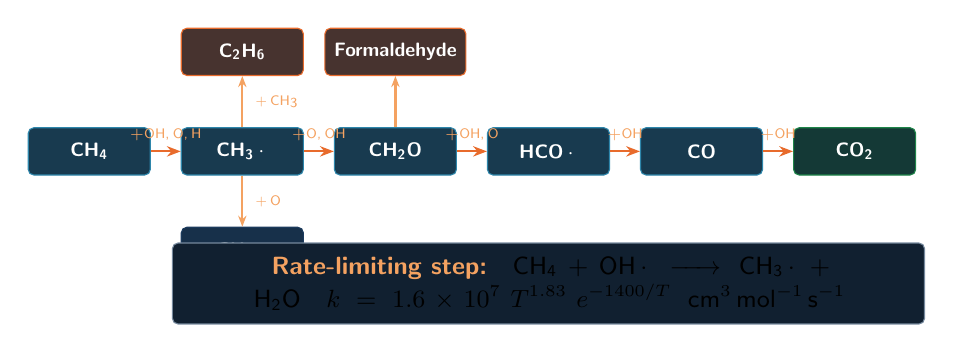
\begin{tikzpicture}[node distance=0.18cm and 0.38cm]
    \node[spSky]                    (ch4)  {\ce{CH4}};
    \node[spSky, right=of ch4]      (ch3)  {\ce{CH3.}};
    \node[spSky, right=of ch3]      (ch2o) {\ce{CH2O}};
    \node[spSky, right=of ch2o]     (hco)  {\ce{HCO.}};
    \node[spSky, right=of hco]      (co)   {\ce{CO}};
    \node[spGreen, right=of co]     (co2)  {\ce{CO2}};

    \draw[rxnarrow] (ch4)  -- node[above,lbl]{$+$\ce{OH,O,H}} (ch3);
    \draw[rxnarrow] (ch3)  -- node[above,lbl]{$+$\ce{O,OH}}   (ch2o);
    \draw[rxnarrow] (ch2o) -- node[above,lbl]{$+$\ce{OH,O}}   (hco);
    \draw[rxnarrow] (hco)  -- node[above,lbl]{$+$\ce{OH}}     (co);
    \draw[rxnarrow] (co)   -- node[above,lbl]{$+$\ce{OH}}     (co2);

    \node[spOrange, above=0.65cm of ch3]  (c2h6) {\ce{C2H6}};
    \node[spSteel,  below=0.65cm of ch3]  (ch2)  {\ce{CH2.}};
    \draw[downrxn] (ch3.north) -- node[right,lbl]{\ce{+CH3}} (c2h6.south);
    \draw[downrxn] (ch3.south) -- node[right,lbl]{\ce{+O}}   (ch2.north);

    \node[spOrange, above=0.65cm of ch2o] (hcho) {\scriptsize Formaldehyde};
    \draw[downrxn] (ch2o.north) -- (hcho.south);

    \node[boxcard, below=0.85cm of hco, text width=9.2cm, align=center]
      {\small\hl{Rate-limiting step:}\quad
       \ce{CH4 + OH. -> CH3. + H2O}\quad
       $k = 1.6\times10^{7}\ T^{1.83}\ e^{-1400/T}$\;
       cm$^3$\,mol$^{-1}$\,s$^{-1}$};
  \end{tikzpicture}
  \end{center}
\end{frame}

\begin{frame}{\ce{CH4} --- \ce{C2} Sub-mechanism \& Low-Temperature Kinetics}
  \begin{columns}[t]
    \column{0.48\textwidth}
    \begin{block}{\ce{C2} Sub-mechanism (High-$T$)}
      \begin{itemize}
        \item \rxn{\ce{CH3. + CH3. <=> C2H6}}
        \item \rxn{\ce{C2H6 + H./OH. -> C2H5. + H2/H2O}}
        \item \rxn{\ce{C2H5. -> C2H4 + H.}}\ ($\beta$-scission)
        \item \rxn{\ce{C2H4 + O./OH. -> CH3CHO,\;CH2CHO.}}
        \item \ce{C2H2} (acetylene) $\to$ soot precursor path
      \end{itemize}
    \end{block}
    \begin{exampleblock}{Selected Rate Constants}
      \footnotesize
      \begin{tabular}{@{}ll@{}}
        \ce{CH4 + OH} & $k=1.6\!\times\!10^7 T^{1.83} e^{-1400/T}$ \\
        \ce{CH3 + O2} & $k=2.0\!\times\!10^{12} e^{-30480/T}$ \\
        \ce{CO  + OH} & $k=4.76\!\times\!10^7 T^{1.23} e^{35/T}$ \\
      \end{tabular}
    \end{exampleblock}
    \column{0.48\textwidth}
    \begin{alertblock}{Low-$T$ \ce{CH4} Oxidation ($T < 900\,\mathrm{K}$)}
      \begin{enumerate}
        \item \rxn{\ce{CH3. + O2 -> CH3OO.}}
        \item \rxn{\ce{CH3OO. + RH -> CH3OOH + R.}}
        \item \rxn{\ce{CH3OOH -> CH3O. + OH.}}\ (branching)
        \item Chain branching $\to$ ignition
      \end{enumerate}
      \vspace{0.15cm}
      \footnotesize Relevant to HCCI/SACI.
      NTC arises from competing \ce{RO2} isomerisation.
    \end{alertblock}
    \begin{block}{Mechanism Files}
      \begin{itemize}
        \item GRI-Mech 3.0 (53 species, 325 rxns)
        \item AramcoMech 3.0 (\ce{C1}--\ce{C4})
        \item Leeds Methane Mech v1.5
      \end{itemize}
    \end{block}
  \end{columns}
\end{frame}

% ════════════════════════════════════════════════════════════
\section{\texorpdfstring{\ce{H2}}{H2} Oxidation}
% ════════════════════════════════════════════════════════════

\begin{frame}{\ce{H2/O2} Mechanism --- Elementary Reactions}
  \begin{columns}[t]
    \column{0.54\textwidth}
    \small\renewcommand{\arraystretch}{1.25}
    \begin{tabular}{@{}clll@{}}
      \toprule
      \rowcolor{ITUsteel}
      \textbf{\color{white}\#} &
      \textbf{\color{white}Reaction} &
      \textbf{\color{white}Class} \\
      \midrule
      R1  & \ce{H2 + O2 -> HO2. + H.}       & Initiation \\
      \rowcolor{ITUpanel}
      R2  & \ce{H. + O2 -> OH. + O.}         & \redbf{Chain branching} \\
      R3  & \ce{O. + H2 -> OH. + H.}         & Propagation \\
      \rowcolor{ITUpanel}
      R4  & \ce{OH. + H2 -> H2O + H.}        & Propagation \\
      R5  & \ce{H. + O2 + M -> HO2. + M}     & Termination \\
      \rowcolor{ITUpanel}
      R6  & \ce{HO2. + H. -> OH. + OH.}      & \ce{HO2} branching \\
      R7  & \ce{HO2. + H. -> H2 + O2}        & \ce{HO2} termination \\
      \rowcolor{ITUpanel}
      R8  & \ce{OH. + OH. + M -> H2O2 + M}   & \ce{H2O2} formation \\
      R9  & \ce{H2O2 + M -> OH. + OH. + M}   & \ce{H2O2} decomp.\\
      \rowcolor{ITUpanel}
      R10 & \ce{H. + H. + M -> H2 + M}       & Recombination \\
      \bottomrule
    \end{tabular}
    \column{0.43\textwidth}
    \begin{alertblock}{Critical Branching Step}
      \[
        \underbrace{\ce{H. + O2 -> OH. + O.}}_{\text{R2},\;
          E_a = 16.4\,\text{kcal/mol}}
      \]
      \small Competes with R5 (\ce{H. + O2 + M}).\\
      \hl{Explosion} when R2\,$>$\,R5;\\
      determined by $(p,T)$ crossover.
    \end{alertblock}
    \begin{block}{Ignition Properties}
      \footnotesize
      \begin{tabular}{@{}ll@{}}
        Flamm.\ limits & 4--75\,vol\% in air \\
        $T_\text{aut}$  & $\approx500\,^{\circ}$C \\
        Min.\ ign.\ energy & 0.017\,mJ \\
        $S_L$ (stoich.) & 2.9\,m/s \\
        $T_\text{ad}$   & 2480\,K \\
      \end{tabular}
    \end{block}
  \end{columns}
\end{frame}

\begin{frame}{\ce{H2} Explosion Limits \& Special Features}
  \begin{columns}[t]
    \column{0.48\textwidth}
    \begin{block}{\ce{H2/O2} Explosion Limits (schematic)}
    \vspace{-0.1cm}
    \begin{center}
    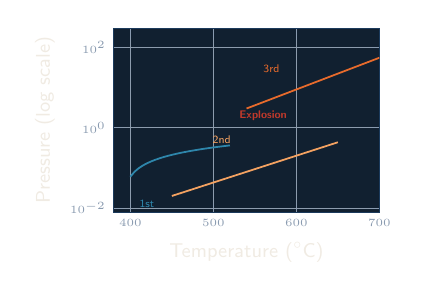
\begin{tikzpicture}[scale=0.80]
      \begin{axis}[
        xlabel={\small Temperature ($^\circ$C)},
        ylabel={\small Pressure (log scale)},
        ymode=log,
        xmin=380, xmax=700,
        ymin=0.008, ymax=300,
        width=5.8cm, height=4.5cm,
        grid=both,
        grid style={draw=ITUsteel!50, very thin},
        axis background/.style={fill=ITUpanel},
        tick style={color=ITUmuted},
        ticklabel style={color=ITUmuted, font=\tiny},
        xlabel style={color=ITUcream, font=\small},
        ylabel style={color=ITUcream, font=\small},
        axis line style={color=ITUsteel},
      ]
        \addplot[thick, color=ITUsky,   domain=400:520]
          ({x}, {0.012*(x-390)^0.7});
        \addplot[thick, color=ITUgold,  domain=450:650]
          ({x}, {0.02*exp((x-450)/65)});
        \addplot[thick, color=ITUorange,domain=540:700]
          ({x}, {3*exp((x-540)/55)});
        \node[font=\tiny, color=ITUsky]    at (axis cs:420, 0.013) {1st};
        \node[font=\tiny, color=ITUgold]   at (axis cs:510, 0.5)   {2nd};
        \node[font=\tiny, color=ITUorange] at (axis cs:570, 30)    {3rd};
        \node[font=\tiny, color=ITUred, align=center]
                                           at (axis cs:560, 2)
          {\bfseries Explosion};
      \end{axis}
    \end{tikzpicture}
    \end{center}
    \end{block}
    \column{0.48\textwidth}
    \begin{block}{Why \ce{H2} Is Different}
      \begin{itemize}
        \item \textbf{No carbon} --- direct \ce{H2O}, zero soot
        \item Highest laminar flame speed of any fuel
        \item High diffusivity: $\mathrm{Le}\!\ll\!1$,
              diffusive instabilities
        \item Dominant radical: \ce{OH.} via R2 branching
        \item \ce{HO2.} \& \ce{H2O2} critical at moderate $T$
      \end{itemize}
    \end{block}
    \begin{alertblock}{NNH Pathway (\ce{H2} Combustion)}
      \[
        \ce{NNH + O. -> N2O + H.}
        \;\;\to\;\;
        \ce{N2O + O. -> 2NO}
      \]
      \footnotesize Notable \ce{NO_x} route even without carbon;\\
      relevant at high-altitude \ce{H2} combustion.
    \end{alertblock}
  \end{columns}
\end{frame}

% ════════════════════════════════════════════════════════════
\section{Aerospace Fuels}
% ════════════════════════════════════════════════════════════

\begin{frame}{Aerospace Fuels --- Composition \& Surrogate Strategy}
  \begin{columns}[t]
    \column{0.48\textwidth}
    \begin{block}{Jet-A / Jet-A1}
      \begin{itemize}
        \item \ce{C8}--\ce{C16} paraffins, naphthenics, aromatics
        \item Average formula: \ce{C12H23} ($H/C \approx 1.9$)
        \item POSF-10325 surrogate:\newline
              \textit{n}-\ce{C10} $+$ \textit{i}\ce{C8} $+$ TMB $+$ \textit{n}-\ce{C12}
        \item Boiling range: 150--280\,$^\circ$C; flash point 38\,$^\circ$C
      \end{itemize}
    \end{block}
    \begin{block}{RP-1 (Rocket Propellant)}
      \begin{itemize}
        \item Naphthenic $+$ paraffinic \ce{C10}--\ce{C14}
        \item Surrogate: \textit{n}-decane + cyclopentane + toluene
        \item LOX/RP-1 O/F $\approx 2.56$; high sooting tendency
        \item Falcon~9, Atlas~V, Saturn~V (F-1 engine)
      \end{itemize}
    \end{block}
    \column{0.48\textwidth}
    \begin{block}{Ethylene \ce{C2H4} (Scramjets)}
      \begin{itemize}
        \item Simple \ce{C2} structure; well-studied kinetics
        \item Fast ignition; high reactivity
        \item \ce{C2H4 -> C2H3. -> C2H2 ->} soot
        \item Mechanism: USC Mech~II (111 species)
      \end{itemize}
    \end{block}
    \begin{exampleblock}{Why Surrogates?}
      \small Real fuels contain \textbf{hundreds} of components.
      Surrogates reproduce ignition delay, flame speed,
      soot volume fraction, and JSR speciation.
    \end{exampleblock}
  \end{columns}
\end{frame}

\begin{frame}{\textit{n}-Alkane Oxidation --- High-Temperature Pathway ($T>1000\,\mathrm{K}$)}
  \vspace{0.1cm}
  \begin{center}
  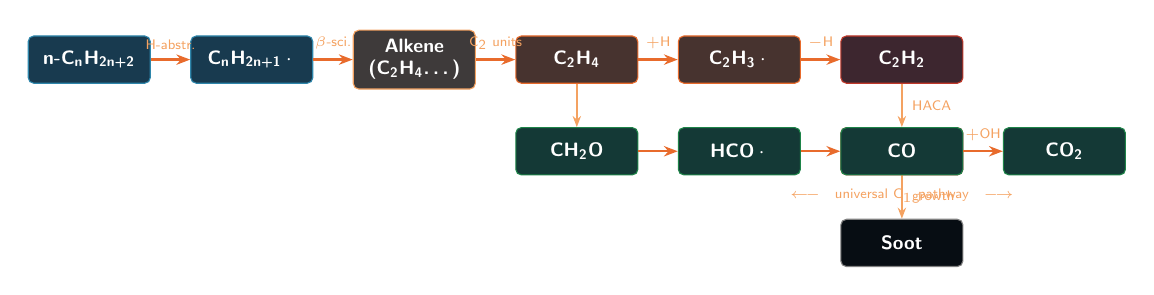
\begin{tikzpicture}[node distance=0.16cm and 0.28cm]
    \node[spSky]                        (alk)   {\scriptsize\textit{n}-\ce{C_nH_{2n+2}}};
    \node[spSky,   right=0.5cm of alk]  (rad)   {\scriptsize\ce{C_nH_{2n+1}.}};
    \node[spGold,  right=0.5cm of rad]  (alkene){\scriptsize Alkene\\\scriptsize(\ce{C2H4}\ldots)};
    \node[spOrange,right=0.5cm of alkene](eth)   {\scriptsize\ce{C2H4}};
    \node[spOrange,right=0.5cm of eth]  (vinyl) {\scriptsize\ce{C2H3.}};
    \node[spRed,   right=0.5cm of vinyl](acet)  {\scriptsize\ce{C2H2}};

    \draw[rxnarrow] (alk)   -- node[above,lbl]{H-abstr.} (rad);
    \draw[rxnarrow] (rad)   -- node[above,lbl]{$\beta$-sci.}(alkene);
    \draw[rxnarrow] (alkene)-- node[above,lbl]{\ce{C2} units}(eth);
    \draw[rxnarrow] (eth)   -- node[above,lbl]{$+$H}      (vinyl);
    \draw[rxnarrow] (vinyl) -- node[above,lbl]{$-$H}      (acet);

    \node[spRed,   below=0.55cm of acet]  (pah)  {PAH};
    \node[spBlack, below=0.55cm of pah]   (soot) {Soot};
    \draw[downrxn] (acet.south)-- node[right,lbl]{HACA}  (pah.north);
    \draw[downrxn] (pah.south) -- node[right,lbl]{growth}(soot.north);

    \node[spGreen, below=0.55cm of eth]          (ch2o2){\scriptsize\ce{CH2O}};
    \node[spGreen, right=0.5cm of ch2o2]         (hco2) {\scriptsize\ce{HCO.}};
    \node[spGreen, right=0.5cm of hco2]          (co_n) {\scriptsize\ce{CO}};
    \node[spGreen, right=0.5cm of co_n]          (co2_n){\scriptsize\ce{CO2}};
    \draw[downrxn] (eth.south) -- (ch2o2.north);
    \draw[rxnarrow](ch2o2)--(hco2);
    \draw[rxnarrow](hco2) --(co_n);
    \draw[rxnarrow](co_n) -- node[above,lbl]{$+$OH}(co2_n);
    \node[below=0.05cm of co_n, font=\tiny, color=ITUgold]
      {$\longleftarrow$\quad universal C$_1$ pathway\quad$\longrightarrow$};
  \end{tikzpicture}
  \end{center}
  \vspace{0.1cm}
  \begin{alertblock}{}
    \centering\small
    All higher-alkane oxidation converges on:\quad
    \ce{CH3. -> CH2O -> HCO. -> CO -> CO2}
  \end{alertblock}
\end{frame}

\begin{frame}{Low-Temperature \textit{n}-Alkane Oxidation \& NTC Behaviour}
  \begin{columns}[t]
    \column{0.56\textwidth}
    \begin{block}{Low-$T$ Mechanism (700--900\,K)}
      \begin{enumerate}\small
        \item \rxn{\ce{R. + O2 <=> ROO.}}\quad(alkylperoxy formation)
        \item \rxn{\ce{ROO. -> QOOH.}}\quad(intramolecular H-transfer)
        \item \rxn{\ce{QOOH. + O2 -> OOQOOH}}\quad(2nd O$_2$ addition)
        \item \rxn{\ce{OOQOOH -> OH. + keto-hydroperoxide}}\quad\redbf{(branching!)}
        \item Keto-hydroperoxide $\to$ 2\,\ce{OH.} $+$ carbonyl radical
      \end{enumerate}
      \smallskip
      \small At $T>900\,\mathrm{K}$:
      \ce{ROO. -> olefin + HO2.}\ (termination)\\[3pt]
      $\Rightarrow$ \hl{NTC: increasing $T$ slows ignition (700--900\,K)}
    \end{block}
    \column{0.41\textwidth}
    \begin{block}{NTC Characteristics}
      \begin{itemize}
        \item $n$-alkanes: pronounced NTC ($\geq$\,\ce{C5})
        \item Iso-alkanes: much weaker NTC
        \item Aromatics: virtually none
        \item RP-1: strong NTC
      \end{itemize}
    \end{block}
    \begin{alertblock}{Engineering Impact}
      \begin{itemize}
        \item HCCI/SACI: two-stage ignition
        \item Engine knock prediction
        \item SAF exploits NTC suppression
        \item Diesel ignition delay modelling
      \end{itemize}
    \end{alertblock}
  \end{columns}
\end{frame}

% ════════════════════════════════════════════════════════════
\section{Pollutant Formation}
% ════════════════════════════════════════════════════════════

\begin{frame}{\ce{NO_x} Formation Pathways}
  \begin{columns}[t]
    \column{0.32\textwidth}
    \begin{alertblock}{Thermal (Zeldovich)}
      \footnotesize
      \begin{align*}
        &\ce{O. + N2 -> NO + N.}\\
        &\ce{N. + O2 -> NO + O.}\\
        &\ce{N. + OH. -> NO + H.}
      \end{align*}
      Dominant at $T>1800\,\mathrm{K}$.\\
      $k\propto e^{-38000/T}$\\
      Very sensitive to peak $T$.
    \end{alertblock}
    \column{0.32\textwidth}
    \begin{block}{Prompt (Fenimore)}
      \footnotesize
      \begin{align*}
        &\ce{CH. + N2 -> HCN + N.}\\
        &\ce{HCN -> CN. -> NO}
      \end{align*}
      In fuel-rich flame front.\\
      Significant at lower $T$.\\
      Important in swirl burners.
    \end{block}
    \column{0.32\textwidth}
    \begin{exampleblock}{\ce{N2O} \& NNH Routes}
      \footnotesize
      \begin{align*}
        &\ce{N2O + O. -> 2NO}\\
        &\ce{NNH + O. -> N2O + H.}
      \end{align*}
      Lean, high-$p$ combustion.\\
      Notable in \ce{H2} flames.\\
      High-altitude relevance.
    \end{exampleblock}
  \end{columns}
  \vspace{0.25cm}
  \begin{block}{Mitigation Strategies in Aerospace Combustion}
    \begin{columns}
      \column{0.48\textwidth}
      \begin{itemize}\small
        \item Lean premixed (LPP/DLE): reduce peak $T$
        \item Staged combustion: rich\,$+$\,lean zones
      \end{itemize}
      \column{0.48\textwidth}
      \begin{itemize}\small
        \item Water/steam injection
        \item \ce{H2} substitution: zero carbon, lower thermal \ce{NO}
      \end{itemize}
    \end{columns}
  \end{block}
\end{frame}

\begin{frame}{Soot Formation: HACA Mechanism}
  \begin{center}
  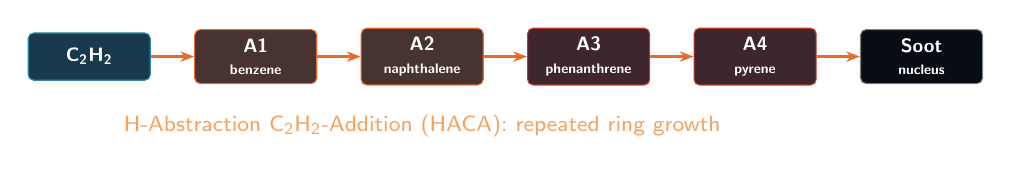
\begin{tikzpicture}[node distance=0.15cm and 0.40cm]
    \node[spSky]                        (c2h2){\ce{C2H2}};
    \node[spOrange, right=0.55cm of c2h2](a1) {A1\\\tiny benzene};
    \node[spOrange, right=0.55cm of a1]  (a2) {A2\\\tiny naphthalene};
    \node[spRed,    right=0.55cm of a2]  (a3) {A3\\\tiny phenanthrene};
    \node[spRed,    right=0.55cm of a3]  (a4) {A4\\\tiny pyrene};
    \node[spBlack,  right=0.55cm of a4]  (soot){Soot\\\tiny nucleus};

    \draw[rxnarrow](c2h2)--(a1);
    \draw[rxnarrow](a1)--(a2);
    \draw[rxnarrow](a2)--(a3);
    \draw[rxnarrow](a3)--(a4);
    \draw[rxnarrow](a4)--(soot);
    \node[below=0.25cm of a2, font=\footnotesize, color=ITUgold]
      {H-Abstraction \ce{C2H2}-Addition (HACA): repeated ring growth};
  \end{tikzpicture}
  \end{center}
  \vspace{0.05cm}
  \begin{columns}[t]
    \column{0.48\textwidth}
    \begin{block}{HACA Steps}
      \begin{enumerate}\small
        \item \ce{ArH + H. -> Ar. + H2}\quad(H-abstraction)
        \item \ce{Ar. + C2H2 -> Ar-CH=CH.}\quad(\ce{C2H2} addition)
        \item Ring closure $\to$ larger PAH
        \item Repeat until pyrene (A4) $\to$ soot inception
        \item Surface HACA $+$ coagulation $\to$ particle growth
      \end{enumerate}
    \end{block}
    \column{0.48\textwidth}
    \begin{alertblock}{Aerospace Relevance}
      \begin{itemize}
        \item RP-1 \& Jet-A: high soot (aromatics\,$+$\,cycloalkanes)
        \item SAF: 50--70\% soot reduction vs.\ Jet-A
        \item \ce{H2}: \textbf{zero soot} --- key sustainability advantage
        \item Soot $\to$ radiation load in rocket chambers
        \item Oxidation: \ce{C + OH -> CO + H}
      \end{itemize}
    \end{alertblock}
  \end{columns}
\end{frame}

% ════════════════════════════════════════════════════════════
\section{Summary}
% ════════════════════════════════════════════════════════════

\begin{frame}{Comparative Summary --- Oxidation Pathways}
  \small\renewcommand{\arraystretch}{1.30}\setlength{\tabcolsep}{4pt}
  \begin{tabular}{@{}llllll@{}}
    \toprule
    \rowcolor{ITUsteel}
    \color{ITUgold}\bfseries Property &
    \color{ITUgold}\bfseries \ce{CH4}  &
    \color{ITUgold}\bfseries \ce{H2}   &
    \color{ITUgold}\bfseries Jet-A     &
    \color{ITUgold}\bfseries RP-1      &
    \color{ITUgold}\bfseries \ce{C2H4} \\
    \midrule
    Mechanism         & GRI-Mech 3.0 & Li/Burke     & POSF surrog.      & \textit{n}-C10 & USC Mech II \\
    \rowcolor{ITUpanel}
    \# Species        & 53           & 9--13        & $\sim$200         & $\sim$200      & 111 \\
    $S_L$ (m/s)       & 0.36         & 2.9          & $\sim$0.40        & $\sim$0.37     & 0.66 \\
    \rowcolor{ITUpanel}
    $T_\text{ad}$ (K) & 2226         & 2480         & $\sim$2270        & $\sim$2250     & 2375 \\
    NTC               & Mild         & None         & Moderate          & Strong         & Weak \\
    \rowcolor{ITUpanel}
    Soot              & Low          & \bfseries Zero & Mod.--High      & High           & High \\
    Key radical       & \ce{OH,CH3}  & \ce{OH,H}    & \ce{OH,H}         & \ce{OH,H}      & \ce{OH,C2H3} \\
    \rowcolor{ITUpanel}
    Key interm.       & \ce{CH2O}    & \ce{HO2}     & Olefins, \ce{CH2O}& Olefins        & \ce{C2H2} \\
    Application       & Gas turbines & \ce{LH2} rockets & Aviation      & Rockets        & Scramjets \\
    \bottomrule
  \end{tabular}
\end{frame}

\begin{frame}{Key Takeaways}
  \setlength{\parskip}{0pt}
  \setbeamerfont{block body}{size=\footnotesize}
  \setbeamerfont{block title}{size=\footnotesize,series=\bfseries}
  {\footnotesize
  \begin{block}{\color{ITUorange}\bfseries 1.\enspace Universal \ce{C1} Convergence}
    All hydrocarbon fuels ultimately oxidise via \ce{CH3. -> CH2O -> HCO. -> CO -> CO2}.
  \end{block}\vspace{-4pt}
  \begin{block}{\color{ITUsky}\bfseries 2.\enspace Radical Chain Control}
    H, O, OH dominate high-$T$; \ce{HO2} and \ce{H2O2} govern low/intermediate $T$.
    Radical pool growth determines $\tau_\text{ign}$ and flame structure.
  \end{block}\vspace{-4pt}
  \begin{block}{\color{ITUgreen}\bfseries 3.\enspace \ce{H2} --- The Simplest Case}
    9 species, no carbon intermediates, extreme reactivity, zero soot.
    Reference for H--O chemistry in all hydrocarbon mechanisms.
  \end{block}\vspace{-4pt}
  \begin{block}{\color{ITUgold}\bfseries 4.\enspace Fuel Structure Matters}
    Branching suppresses NTC; aromatics drive soot; chain length controls
    low-$T$ reactivity. Directly relevant to SAF and propellant design.
  \end{block}\vspace{-4pt}
  \begin{alertblock}{\bfseries 5.\enspace Coupled Pollutant Chemistry}
    \ce{NO_x}, CO, and soot form via competing pathways strongly coupled to
    temperature, equivalence ratio $\phi$, and pressure $p$.
  \end{alertblock}}
\end{frame}

\begin{frame}{References \& Further Reading}
  \begin{columns}[t]
    \column{0.48\textwidth}
    \begin{block}{Textbooks}
      \begin{itemize}
        \item Turns, S.R.\ \textit{An Introduction to Combustion}, 3rd~ed.
        \item Williams, F.A.\ \textit{Combustion Theory}, 2nd~ed.
        \item Law, C.K.\ \textit{Combustion Physics}
        \item Kuo, K.K.\ \textit{Principles of Combustion}, 2nd~ed.
      \end{itemize}
    \end{block}
    \begin{exampleblock}{Mechanisms}
      \begin{itemize}
        \item GRI-Mech 3.0 --- \texttt{me.berkeley.edu/gri\_mech}
        \item AramcoMech 3.0 --- NUI Galway
        \item LLNL \textit{n}/\textit{iso}-alkane mechanisms
        \item USC Mech~II (\ce{C1}--\ce{C4}\,$+$\,\ce{H2/CO})
      \end{itemize}
    \end{exampleblock}
    \column{0.48\textwidth}
    \begin{block}{Key Papers}
      \begin{itemize}
        \item Westbrook \& Dryer (1984), \textit{Combust.\ Flame}
        \item Curran et al.\ (2002) --- low-$T$ \textit{n}-heptane/iC8
        \item Li et al.\ (2004) --- \ce{H2/O2} mechanism
        \item Metcalfe et al.\ (2013) --- AramcoMech~1.3
        \item Dooley et al.\ (2012) --- Jet-A surrogate
      \end{itemize}
    \end{block}
    \begin{alertblock}{Software \& Databases}
      \begin{itemize}
        \item Cantera (Python/C++) --- \texttt{cantera.org}
        \item CHEMKIN-Pro / OpenSMOKE++
        \item NIST Chemistry WebBook
        \item ReSpecTh / PrIMe databases
      \end{itemize}
    \end{alertblock}
  \end{columns}
\end{frame}

% ── CLOSING SLIDE ───────────────────────────────────────────
{
\setbeamertemplate{footline}{}
\begin{frame}[plain]
  \begin{tikzpicture}[remember picture,overlay]
    \fill[ITUnavy] (current page.south west) rectangle (current page.north east);
    \fill[ITUorange] (current page.north west)
      rectangle ([xshift=0.55cm]current page.south west);
    \fill[ITUgold!70!ITUorange] ([xshift=0.55cm]current page.north west)
      rectangle ([xshift=0.72cm]current page.south west);
    \fill[ITUsteel] ([yshift=0.45cm]current page.south west)
      rectangle (current page.south east);
  \end{tikzpicture}
  \vspace{0.6cm}
  \hspace{1.0cm}%
  \begin{minipage}{0.82\textwidth}
    {\color{white}\huge\bfseries Questions?}\par
    \vspace{0.4cm}
    {\color{ITUgold}\large\itshape Discussion \& Problem Session}\par
    \vspace{0.8cm}
    {\color{ITUmuted}\small Next lecture: Plug Flow Reactors }\par
    \vspace{0.8cm}
    {\color{ITUmuted}\footnotesize Istanbul Technical University
     $\cdot$ UCK 427E Combustion}
  \end{minipage}
\end{frame}
}

\end{document}
